
% ---- fig000_eser.pgf ----
% (c) 2012 Dimitrios Vrettos - d.vrettos@gmail.com
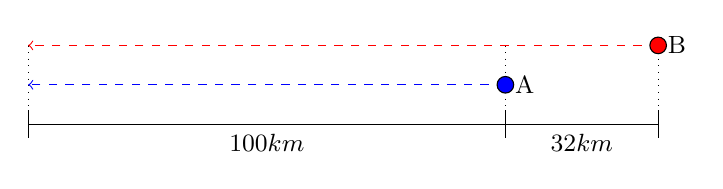
\begin{tikzpicture}[font=\small,x=10mm, y=10mm]
\draw (0,0) -- (8,0);
\foreach \x in {0,6.06,8}{
\draw (\x,5pt) -- (\x,-5pt);
\draw[dotted] (\x,1) -- (\x,0);
}

\draw[dashed, red, ->] (8,1) -- (0,1);
\draw[dashed, blue, ->] (6.06,.5) -- (0,.5);

\draw[fill=blue] (6.06,.5) circle (3pt) node [right] () {A};
\draw[fill=red] (8,1) circle (3pt) node [right] () {B};

\node[below] at (3.03,0) {$100\munit{km}$};
\node[below] at (7.03,0) {$32\munit{km}$};
\end{tikzpicture}
% -----------------

% ---- fig0010_eser.pgf ----
% (c) 2012 Dimitrios Vrettos - d.vrettos@gmail.com
\begin{tikzpicture}[font=\small,x=10mm, y=5mm]

\draw[->] (0,0) -- (8,0) node [below right] () {$r$};
\node[above]  at (2,0) {$-2$};
\node[above]  at (6,0) {2};
\begin{scope}[blue,thick]
\draw (2,0) -- (6,0);
\foreach \x in {2,6}
\draw[fill=white] (\x,0)circle (1.5pt);
\end{scope}

\end{tikzpicture}% -----------------

% ---- fig001_ret.pgf ----
% (c) 2012 Dimitrios Vrettos - d.vrettos@gmail.com
\begin{tikzpicture}[font=\small,x=10mm, y=5mm]

\draw[->] (0,0) -- (8,0) node [below right] () {$r$};
\node[above]  at (4,0) {3};
\begin{scope}[blue,thick]
\draw (0,0) -- (4,0);
\draw[fill=white] (4,0)circle (1.5pt);
\end{scope}

\end{tikzpicture}% -----------------

% ---- fig002_ret.pgf ----
% (c) 2012 Dimitrios Vrettos - d.vrettos@gmail.com
\begin{tikzpicture}[font=\small,x=10mm, y=5mm]

\draw[->] (0,0) -- (8,0) node [below right] () {$r$};
\node[above]  at (4,0) {$-5$};
\begin{scope}[blue,thick,->]
\draw (4,0) -- (8,0);
\draw[fill=blue] (4,0)circle (1.5pt);
\end{scope}

\end{tikzpicture}% -----------------

% ---- fig003_ret.pgf ----
% (c) 2012 Dimitrios Vrettos - d.vrettos@gmail.com
\begin{tikzpicture}[font=\small,x=10mm, y=5mm]

\draw[->] (0,0) -- (8,0) node [below right] () {$r$};
\node[above]  at (1,0) {$-2$};
\node[above]  at (7,0) {6};
\begin{scope}[blue,thick]
\draw (1,0) -- (7,0);
\foreach \x in {1,7}
\draw[fill=white] (\x,0)circle (1.5pt);
\end{scope}

\end{tikzpicture}% -----------------

% ---- fig004_ret.pgf ----
% (c) 2012 Dimitrios Vrettos - d.vrettos@gmail.com
\begin{tikzpicture}[font=\small,x=10mm, y=5mm]

\draw[->] (0,0) -- (8,0) node [below right] () {$r$};
\node[above]  at (1,0) {$-2$};
\node[above]  at (7,0) {6};
\begin{scope}[blue,thick]
\draw (1,0) -- (7,0);
\draw[fill=white] (1,0)circle (1.5pt);
\draw[fill=blue] (7,0)circle (1.5pt);
\end{scope}

\end{tikzpicture}% -----------------

% ---- fig005_ret.pgf ----
% (c) 2012 Dimitrios Vrettos - d.vrettos@gmail.com
\begin{tikzpicture}[font=\small,x=10mm, y=5mm]

\draw[->] (0,0) -- (8,0) node [below right] () {$r$};
\node[above]  at (1,0) {$-2$};
\node[above]  at (7,0) {6};
\begin{scope}[blue,thick]
\draw (1,0) -- (7,0);
\foreach \x in {1,7}
\draw[fill=blue] (\x,0)circle (1.5pt);
\end{scope}

\end{tikzpicture}% -----------------

% ---- fig006_ret.pgf ----
% (c) 2012 Dimitrios Vrettos - d.vrettos@gmail.com
\begin{tikzpicture}[font=\small,x=10mm, y=5mm]

\draw[->] (0,0) -- (8,0) node [below right] () {$r$};
\node[above]  at (4,0) {0};
\begin{scope}[blue,thick,->]
\draw (4,0) -- (8,0);
\draw[fill=white] (4,0)circle (1.5pt);
\end{scope}

\end{tikzpicture}% -----------------

% ---- fig007_ret.pgf ----
% (c) 2012 Dimitrios Vrettos - d.vrettos@gmail.com
\begin{tikzpicture}[font=\small,x=10mm, y=5mm]

\draw[->] (0,0) -- (8,0) node [below right] () {$r$};
\node[above]  at (4,0) {0};
\begin{scope}[blue,thick]
\draw (0,0) -- (4,0);
\draw[fill=white] (4,0)circle (1.5pt);
\end{scope}

\end{tikzpicture}% -----------------

% ---- fig008_eser.pgf ----
% (c) 2012 Dimitrios Vrettos - d.vrettos@gmail.com
\begin{tikzpicture}[font=\small,x=10mm, y=5mm]

\draw[->] (0,0) -- (8,0) node [below right] () {$r$};
\node[above]  at (4,0) {$-3$};
\begin{scope}[blue,thick]
\draw (0,0) -- (4,0);
\draw[fill=white] (4,0)circle (1.5pt);
\end{scope}

\end{tikzpicture}% -----------------

% ---- fig009_eser.pgf ----
% (c) 2012 Dimitrios Vrettos - d.vrettos@gmail.com
\begin{tikzpicture}[font=\small,x=10mm, y=5mm]

\draw[->] (0,0) -- (8,0) node [below right] () {$r$};
\node[above]  at (4,0) {$2$};
\begin{scope}[blue,thick,->]
\draw (4,0) -- (8,0);
\draw[fill=blue] (4,0)circle (1.5pt);
\end{scope}

\end{tikzpicture}% -----------------

% ---- fig010_eser.pgf ----
% (c) 2012 Dimitrios Vrettos - d.vrettos@gmail.com
\begin{tikzpicture}[font=\small,x=10mm, y=5mm]

\draw[->] (0,0) -- (8,0) node [below right] () {$r$};
\node[above]  at (2,0) {$-2$};
\node[above]  at (6,0) {2};
\begin{scope}[blue,thick]
\draw (2,0) -- (6,0);
\foreach \x in {2,6}
\draw[fill=white] (\x,0)circle (1.5pt);
\end{scope}

\end{tikzpicture}% -----------------

% ---- fig011_eser.pgf ----
% (c) 2012 Dimitrios Vrettos - d.vrettos@gmail.com
\begin{tikzpicture}[font=\small,x=10mm, y=5mm]

\draw[->] (0,0) -- (8,0) node [below right] () {$r$};
\node[above]  at (2,0) {$3$};
\node[above]  at (6,0) {5};
\begin{scope}[blue,thick]
\draw (2,0) -- (6,0);
\draw[fill=white] (2,0)circle (1.5pt);
\draw[fill=blue] (6,0)circle (1.5pt);
\end{scope}

\end{tikzpicture}% -----------------

% ---- fig012_eser.pgf ----
% (c) 2012 Dimitrios Vrettos - d.vrettos@gmail.com
\begin{tikzpicture}[font=\small,x=10mm, y=5mm]

\draw[->] (0,0) -- (8,0) node [below right] () {$r$};
\node[above]  at (2,0) {$-1$};
\node[above]  at (6,0) {0};
\begin{scope}[blue,thick]
\draw (2,0) -- (6,0);
\draw[fill=blue] (2,0)circle (1.5pt);
\draw[fill=blue] (6,0)circle (1.5pt);
\end{scope}

\end{tikzpicture}% -----------------

% ---- fig013_eser.pgf ----
% (c) 2012 Dimitrios Vrettos - d.vrettos@gmail.com
\begin{tikzpicture}[font=\small,x=10mm, y=5mm]

\draw[->] (0,0) -- (8,0) node [below right] () {$r$};
\node[above]  at (2,0) {$1$};
\node[above]  at (6,0) {2};
\begin{scope}[blue,thick]
\draw (2,0) -- (6,0);
\draw[fill=blue] (2,0)circle (1.5pt);
\draw[fill=white] (6,0)circle (1.5pt);
\end{scope}

\end{tikzpicture}% -----------------

% ---- fig014_ret.pgf ----
% (c) 2012 Dimitrios Vrettos - d.vrettos@gmail.com
\begin{tikzpicture}[font=\small,x=10mm, y=5mm]

\draw[->] (0,0) -- (8,0) node [below right] () {$r$};
\node[above]  at (4,0) {6};
\begin{scope}[blue,thick,->]
\draw (4,0) -- (8,0);
\draw[fill=white] (4,0)circle (1.5pt);
\end{scope}

\end{tikzpicture}% -----------------

% ---- fig015_ret.pgf ----
% (c) 2012 Dimitrios Vrettos - d.vrettos@gmail.com
\begin{tikzpicture}[font=\small,x=10mm, y=5mm]

\draw[->] (0,0) -- (8,0) node [below right] () {$r$};
\node[above]  at (4,0) {$-2$};
\begin{scope}[blue,thick]
\draw (0,0) -- (4,0);
\draw[fill=white] (4,0)circle (1.5pt);
\end{scope}

\end{tikzpicture}% -----------------

% ---- fig016_is.pgf ----
% (c) 2012 Dimitrios Vrettos - d.vrettos@gmail.com
\begin{tikzpicture}[font=\small,x=10mm, y=10mm]

\draw[->] (0,0) -- (8,0) node [below right] () {$r$};

\foreach \x in {2,6}
\draw(\x,3pt)--(\x,-3pt);

\node[above]  at (2,0) {$0$};
\node[above]  at (6,0) {2};

\begin{scope}[dotted]
\draw (2,0) -- (2,-1.5);
\draw (6,0) -- (6,-1.5);
\draw (0,-.5) -- (2,-.5);
\draw (6,-.5) -- (8,-.5);
\end{scope}

\pattern[pattern= north east lines, pattern color=red] (2,-2) rectangle (6,-1.5);

\node[below] () at (4,-2) {$\IS$};

\begin{scope}[blue,thick]
\draw (2,-.5) -- (8,-.5);
\draw (0,-1) -- (6,-1);
\draw[fill=blue] (6,-1)circle (1.5pt);
\draw[fill=white] (2,-.5)circle (1.5pt);
\end{scope}

\end{tikzpicture}% -----------------

% ---- fig017_tri.pgf ----
% (c) 2012 Dimitrios Vrettos - d.vrettos@gmail.com
\begin{tikzpicture}[font=\small,x=10mm, y=10mm]

\draw (0,0) -- (2,3)--(6,0)--(0,0);

\node[left] at (0,0) {$A$};
\node[right] at (6,0) {$B$};
\node[above] at (2,3) {$C$};
\end{tikzpicture}% -----------------

% ---- fig018_is.pgf ----
% (c) 2012 Dimitrios Vrettos - d.vrettos@gmail.com
\begin{tikzpicture}[font=\small,x=10mm, y=10mm]

\draw[->] (-1.5,0) -- (8,0) node [below right] () {$r$};

\foreach \x in {0,1,7}{
\draw(\x,3pt)--(\x,-3pt);
\begin{scope}[dotted]
\draw (\x,0) -- (\x,-2);
\draw (-1.5,-.5) -- (0,-.5);
\draw (-1.5,-1) -- (1,-1);
\draw (7,-1.5) -- (8,-1.5);
\end{scope}}

\node[above]  at (0,0) {$0$};
\node[above]  at (1,0) {$\frac{11}{2}$};
\node[above]  at (7,0) {$\frac{85}{2}$};
\pattern[pattern= north east lines, pattern color=red] (1,-2) rectangle (7,-1.5);

\node[below] () at (4,-2) {$\IS$};

\begin{scope}[blue,thick]
\draw (0,-.5) -- (8,-.5);
\draw (1,-1) -- (8,-1);
\draw (-1.5,-1.5) -- (7,-1.5);

\draw[fill=white] (0,-.5)circle (1.5pt);
\draw[fill=white] (1,-1)circle (1.5pt);
\draw[fill=blue] (7,-1.5)circle (1.5pt);

\end{scope}

\end{tikzpicture}% -----------------

% ---- fig019_is.pgf ----
% (c) 2012 Dimitrios Vrettos - d.vrettos@gmail.com
\begin{tikzpicture}[font=\small,x=10mm, y=10mm]

\draw[->] (0,0) -- (8,0) node [below right] () {$r$};

\foreach \x in {2,6}{
\draw(\x,3pt)--(\x,-3pt);
\begin{scope}[dotted]
\draw (\x,0) -- (\x,-1.5);
\draw (0,-.5) -- (2,-.5);
\draw (0,-1) -- (6,-1);
\end{scope}}

\node[above]  at (2,0) {$-21$};
\node[above]  at (6,0) {$\frac{27}{10}$};
\pattern[pattern= north east lines, pattern color=red] (6,-1) rectangle (8,-1.5);

\node[below] () at (7,-1.5) {$\IS$};

\begin{scope}[blue,thick]
\draw (2,-.5) -- (8,-.5);
\draw (6,-1) -- (8,-1);

\draw[fill=white] (2,-.5)circle (1.5pt);
\draw[fill=white] (6,-1)circle (1.5pt);

\end{scope}

\end{tikzpicture}% -----------------

% ---- fig020_is.pgf ----
% (c) 2012 Dimitrios Vrettos - d.vrettos@gmail.com
\begin{tikzpicture}[font=\small,x=10mm, y=10mm]

\draw[->] (0,0) -- (8,0) node [below right] () {$r$};

\draw(4,3pt)--(4,-3pt);

\begin{scope}[dotted]
\draw (4,0) -- (4,-1.5);
\draw (0,-.5) -- (2,-.5);
\draw (0,-1) -- (4,-1);
\end{scope}

\node[above]  at (4,0) {$0$};
\pattern[pattern= north east lines, pattern color=red] (4,-1) rectangle (8,-1.5);

\node[below] () at (6,-1.5) {$IS$};

\begin{scope}[blue,thick]
\draw (0,-.5) -- (8,-.5);
\draw (4,-1) -- (8,-1);

\draw[fill=white] (4,-1)circle (1.5pt);

\end{scope}

\end{tikzpicture}% -----------------

% ---- fig021_is.pgf ----
% (c) 2012 Dimitrios Vrettos - d.vrettos@gmail.com
\begin{tikzpicture}[font=\small,x=10mm, y=10mm]

\draw[->] (0,0) -- (8,0) node [below right] () {$r$};

\foreach \x in {2,5}{
\draw(\x,3pt)--(\x,-3pt);
\begin{scope}[dotted]
\draw (\x,0) -- (\x,-1.5);
\draw (0,-.5) -- (5,-.5);
\draw (2,-1) -- (8,-1);
\end{scope}}

\node[above]  at (5,0) {$-1$};
\node[above]  at (2,0) {$-\frac{13}{10}$};

\begin{scope}[blue,thick]
\draw (5,-.5) -- (8,-.5);
\draw (0,-1) -- (2,-1);

\draw[fill=blue] (5,-.5)circle (1.5pt);
\draw[fill=blue] (2,-1)circle (1.5pt);

\end{scope}

\end{tikzpicture}% -----------------

% ---- fig024_ret.pgf ----
% (c) 2012 Dimitrios Vrettos - d.vrettos@gmail.com
\begin{tikzpicture}[font=\small,x=10mm, y=10mm]

\draw[->] (0,0) -- (8,0) node [below right] () {$r$};
\draw[dotted] (4,0) -- (4,-.5);

\draw(4,3pt)--(4,-3pt);

\node[above]  at (4,0) {$\frac{7}{3}$};
\begin{scope}[below]
\node at (6,0) {$+$};
\node at (2,0) {$-$};
\end{scope}
\begin{scope}[blue,thick,->]
\draw (4,0) -- (8,0);
\draw[fill=white] (4,0)circle (1.5pt);
\end{scope}

\end{tikzpicture}% -----------------

% ---- fig025_seg.pgf ----
% (c) 2012 Dimitrios Vrettos - d.vrettos@gmail.com
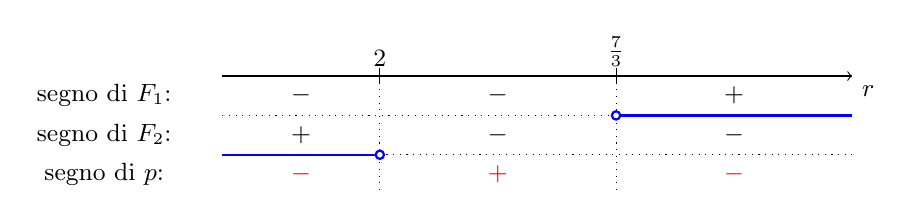
\begin{tikzpicture}[font=\small,x=10mm, y=10mm]

\draw[->] (0,0) -- (8,0) node [below right] () {$r$};

\foreach \x in {2,5}{
\draw(\x,3pt)--(\x,-3pt);
\begin{scope}[dotted]
\draw (\x,0) -- (\x,-1.5);
\draw (0,-.5) -- (5,-.5);
\draw (2,-1) -- (8,-1);
\end{scope}}

\node[above]  at (2,0) {$2$};
\node[above]  at (5,0) {$\frac{7}{3}$};

\begin{scope}[blue,thick]
\draw (5,-.5) -- (8,-.5);
\draw (0,-1) -- (2,-1);

\draw[fill=white] (5,-.5)circle (1.5pt);
\draw[fill=white] (2,-1)circle (1.5pt);
\end{scope}

\foreach \x in {-1.5}{
\node  at (\x,-.25) {segno di $F_1$:};
\node  at (\x,-.75) {segno di $F_2$:};
\node  at (\x,-1.25) {segno di $p$:};
}
\foreach \z in {1,3.5}{
\node  at (\z,-.25) {$-$};
}
\foreach \zi in {3.5, 6.5}{
\node  at (\zi,-.75) {$-$};
}

\node  at (6.5,-.25) {$+$};
\node  at (1,-.75) {$+$};

\begin{scope}[red]
\foreach \zii in {1, 6.5}{
\node  at (\zii,-1.25) {$-$};
}
\node  at (3.5,-1.25) {$+$};
\end{scope}
\end{tikzpicture}
% -----------------

% ---- fig026_seg.pgf ----
% (c) 2012 Dimitrios Vrettos - d.vrettos@gmail.com
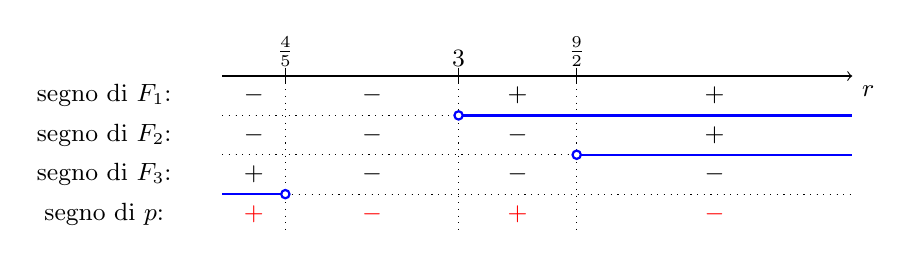
\begin{tikzpicture}[font=\small,x=10mm, y=10mm]

  \draw[->] (0,0) -- (8,0) node [below right] () {$r$};

  \foreach \x in {.8,3,4.5}{
    \draw(\x,3pt)--(\x,-3pt);

  \begin{scope}[dotted]
    \draw (\x,0) -- (\x,-2);
    \draw (0,-.5) -- (3,-.5);
    \draw (0,-1) -- (4.5,-1);
    \draw (.8,-1.5) -- (8,-1.5);
  \end{scope}}

  \node[above] at (.8,0) {$\frac{4}{5}$};
  \node[above]  at (3,0) {$3$};
  \node[above]  at (4.5,0) {$\frac{9}{2}$};

  \begin{scope}[blue,thick]
    \draw (3,-.5) -- (8,-.5);
    \draw (4.5,-1) -- (8,-1);
    \draw (0,-1.5) -- (.8,-1.5);

    \draw[fill=white] (3,-.5)circle (1.5pt);
    \draw[fill=white] (4.5,-1)circle (1.5pt);
    \draw[fill=white] (.8,-1.5)circle (1.5pt);
  \end{scope}

  \foreach \x in {-1.5}{
    \node  at (\x,-.25) {segno di $F_1$:};
    \node  at (\x,-.75) {segno di $F_2$:};
    \node  at (\x,-1.25) {segno di $F_3$:};
    \node  at (\x,-1.75) {segno di $p$:};
  }
  
  \foreach \z in {.4,1.9}
    \node  at (\z,-.25) {$-$};
  
  \foreach \zi in {.4,1.9, 3.75}
    \node  at (\zi,-.75) {$-$};

  \foreach \zii in {1.9, 3.75,6.25}
    \node  at (\zii,-1.25) {$-$};

  \foreach \ziii in {3.75,6.25}
    \node  at (\ziii,-.25) {$+$};

    \node  at (6.25,-.75) {$+$};
    \node  at (.4,-1.25) {$+$};

  \begin{scope}[red]
    \foreach \y in {-1.75}{
      \foreach \ziv in {.4,3.75}
	\node at (\ziv,\y) {$+$};
      \foreach \zv in {1.9,6.25}
	\node at (\zv,\y) {$-$};
      }
  \end{scope}
\end{tikzpicture}% -----------------

% ---- fig027_seg.pgf ----
% (c) 2012 - 2013 Dimitrios Vrettos - d.vrettos@gmail.com
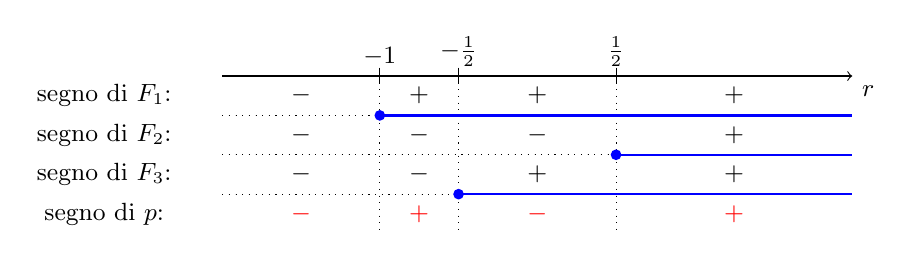
\begin{tikzpicture}[font=\small,x=10mm, y=10mm]

  \draw[->] (0,0) -- (8,0) node [below right] () {$r$};

  \foreach \x in {2,3,5}{
    \draw(\x,3pt)--(\x,-3pt);
    \begin{scope}[dotted]
      \draw (\x,0) -- (\x,-2);
      \draw (0,-.5) -- (2,-.5);
      \draw (0,-1) -- (5,-1);
      \draw (0,-1.5) -- (3,-1.5);
    \end{scope}}

  \node[above]  at (2,0) {$-1$};
  \node[above] at (3,0) {$-\frac{1}{2}$};
  \node[above]  at (5,0) {$\frac{1}{2}$};

  \begin{scope}[blue,thick]
    \draw (2,-.5) -- (8,-.5);
    \draw (5,-1) -- (8,-1);
    \draw (3,-1.5) -- (8,-1.5);

    \draw[fill=blue] (2,-.5)circle (1.5pt);
    \draw[fill=blue] (5,-1)circle (1.5pt);
    \draw[fill=blue] (3,-1.5)circle (1.5pt);
  \end{scope}

  \foreach \x in {-1.5}{
    \node  at (\x,-.25) {segno di $F_1$:};
    \node  at (\x,-.75) {segno di $F_2$:};
    \node  at (\x,-1.25) {segno di $F_3$:};
    \node  at (\x,-1.75) {segno di $p$:};}
  
  \foreach \z in {2.5,4,6.5}
    \node  at (\z,-.25) {$+$};
  
  \foreach \zi in {1,2.5, 4}
    \node  at (\zi,-.75) {$-$};
    
  \foreach \zii in {1,2.5}
    \node  at (\zii,-1.25) {$-$};
  

  \foreach \ziii in {4,6.5}
    \node  at (\ziii,-1.25) {$+$};

  \node  at (1,-.25) {$-$};
  \node  at (6.5,-.75) {$+$};


  \begin{scope}[red]
  \foreach \y in {-1.75}{
    \foreach \ziv in {2.5,6.5}
      \node at (\ziv,\y) {$+$};
    \foreach \zv in {1,4}
      \node at (\zv,\y) {$-$};
  }
  \end{scope}
\end{tikzpicture}
% -----------------

% ---- fig028_seg.pgf ----
% (c) 2012 Dimitrios Vrettos - d.vrettos@gmail.com
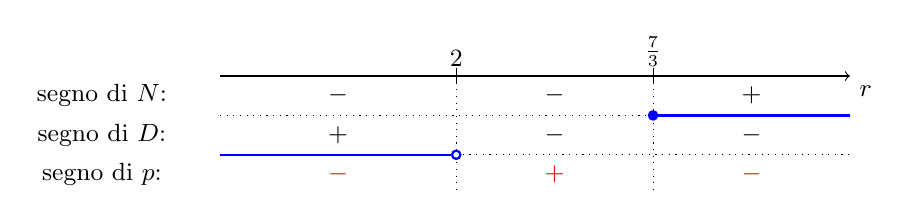
\begin{tikzpicture}[font=\small,x=10mm, y=10mm]

\draw[->] (0,0) -- (8,0) node [below right] () {$r$};

\foreach \x in {3,5.5}{
\draw(\x,3pt)--(\x,-3pt);
\begin{scope}[dotted]
\draw (\x,0) -- (\x,-1.5);
\draw (0,-.5) -- (5.5,-.5);
\draw (3,-1) -- (8,-1);
\end{scope}}

\node[above]  at (3,0) {$2$};
\node[above]  at (5.5,0) {$\frac{7}{3}$};

\begin{scope}[blue,thick]
\draw (5.5,-.5) -- (8,-.5);
\draw (3,-1) -- (0,-1);

\draw[fill=blue] (5.5,-.5)circle (1.5pt);
\draw[fill=white] (3,-1)circle (1.5pt);
\end{scope}

\foreach \x in {-1.5}{
\node  at (\x,-.25) {segno di $N$:};
\node  at (\x,-.75) {segno di $D$:};
\node  at (\x,-1.25) {segno di $p$:};
}
\foreach \z in {1.5,4.25}
\node  at (\z,-.25) {$-$};

\foreach \zi in {4.25,6.75}
\node  at (\zi,-.75) {$-$};

\node  at (6.75,-.25) {$+$};
\node  at (1.5,-.75) {$+$};

\begin{scope}[red]
\foreach \y in {-1.25}{
\foreach \ziv in {4.25}
	\node at (\ziv,\y) {$+$};
\foreach \zv in {1.5,6.75}
\node at (\zv,\y) {$-$};
}
\end{scope}
\end{tikzpicture}% -----------------

% ---- fig029_seg.pgf ----
% (c) 2012 Dimitrios Vrettos - d.vrettos@gmail.com
\begin{tikzpicture}[font=\small,x=10mm, y=10mm]

  \draw[->] (0,0) -- (8,0) node [below right] () {$r$};

  \foreach \x in {1.5,2.75,3.75,5.75}{
    \draw(\x,3pt)--(\x,-3pt);
    
    \begin{scope}[dotted]
      \draw (\x,0) -- (\x,-2.5);
      \draw (0,-.5) -- (3.75,-.5);
      \draw (0,-1) -- (1.5,-1);
      \draw (0,-1.5) -- (5.75,-1.5);
      \draw (0,-2) -- (2.75,-2);
    \end{scope}
  }

  \node[above]  at (1.5,0) {$-1$};
  \node[above] at (2.75,0) {$-\frac{1}{2}$};
  \node[above]  at (3.75,0) {$-\frac{1}{4}$};
  \node[above]  at (5.75,0) {$\frac{1}{2}$};

  \begin{scope}[blue,thick]
    \draw (3.75,-.5) -- (8,-.5);
    \draw (1.5,-1) -- (8,-1);
    \draw (5.75,-1.5) -- (8,-1.5);
    \draw (2.75,-2) -- (8,-2);

    \draw[fill=white] (3.75,-.5)circle (1.5pt);
    \draw[fill=white] (1.5,-1)circle (1.5pt);
    \draw[fill=white] (5.75,-1.5)circle (1.5pt);
    \draw[fill=white] (2.75,-2)circle (1.5pt);
  \end{scope}

  \foreach \x in {-1.5}{
    \node  at (\x,-.25) {segno di $N$:};
    \node(d1)  at (\x,-.75) {segno di $d_1$:};
    \node  at (\x,-1.25) {segno di $d_2$:};
    \node (d3) at (\x,-1.75) {segno di $d_3$:};
    \node  at (\x,-2.25) {segno di $f$:};
    }

  \draw[decorate, decoration={brace, mirror}] let \p1=(d1.north west), \p2=(d3.south west) in(\p1 ) -- (\p2) node[midway, left=2pt] {$D:$};

  \foreach \z in {.75, 2.125,3.25}
    \node  at (\z,-.25) {$-$};

  \foreach \zi in {4.75, 6.875}
    \node  at (\zi,-.25) {$+$};

  \foreach \zii in {2.125,3.25,4.75, 6.875}
    \node  at (\zii,-.75) {$+$};

  \foreach \ziii in {.75,2.125,3.25,4.75}
    \node  at (\ziii,-1.25) {$-$};

  \foreach \ziv in {.75,2.125}
    \node at (\ziv,-1.75) {$-$};

  \foreach \zv in {3.25,4.75, 6.875}
    \node at (\zv,-1.75) {$+$};

  \node  at (.75,-.75) {$-$};
  \node  at (6.875,-1.25) {$+$};

  \begin{scope}[red]
    \foreach \y in {-2.25}{
      \foreach \ziv in {.75,3.25,6.875}
	\node at (\ziv,\y) {$+$};
      \foreach \zv in {2.125,4.75}
	\node at (\zv,\y) {$-$};
    }
  \end{scope}
\end{tikzpicture}% -----------------

% ---- fig030_seg.pgf ----
% (c) 2012 Dimitrios Vrettos - d.vrettos@gmail.com
\begin{tikzpicture}[font=\small,x=10mm, y=10mm]

\draw[->] (0,0) -- (8,0) node [below right] () {$r$};

\foreach \x in {1,3.72,5.56}{
\draw(\x,3pt)--(\x,-3pt);
\begin{scope}[dotted]
\draw (\x,0) -- (\x,-2);
\draw (0,-.5) -- (1,-.5);
\draw (0,-1) -- (5.56,-1);
\draw (0,-1.5) -- (3.72,-1.5);

\end{scope}}


\node[above] at (1,0) {$\frac{2}{11}$};
\node[above]  at (3.72,0) {$\frac{2}{3}$};
\node[above]  at (5.56,0) {$1$};

\begin{scope}[blue,thick]
\draw (1,-.5) -- (8,-.5);
\draw (5.56,-1) -- (8,-1);
\draw (3.72,-1.5) -- (8,-1.5);

\draw[fill=blue] (1,-.5)circle (1.5pt);
\draw[fill=white] (5.56,-1)circle (1.5pt);
\draw[fill=white] (3.72,-1.5)circle (1.5pt);
\end{scope}

\foreach \x in {-1.5}{
\node  at (\x,-.25) {segno di $N$:};
\node(d1)  at (\x,-.75) {segno di $d_1$:};
\node (d2) at (\x,-1.25) {segno di $d_2$:};
\node (d3) at (\x,-1.75) {segno di $f$:};
}

 \draw[decorate, decoration={brace, mirror}]  let \p1=(d1.north west), \p2=(d2.south west) in(\p1 ) -- (\p2) node[midway, left=2pt] {$D:$};

\foreach \z in {2.36,4.64,6.78}
\node  at (\z,-.25) {$+$};

 \foreach \zi in {.5,2.36,4.64}
 \node  at (\zi,-.75) {$-$};

\foreach \zii in {.5,2.36}
 \node  at (\zii,-1.25) {$-$};

 \foreach \ziii in {4.64,6.78}
\node  at (\ziii,-1.25) {$+$};

\node  at (.5,-.25) {$-$};
\node  at (6.78,-.75) {$+$};

\begin{scope}[red]
\foreach \y in {-1.75}{
\foreach \ziv in {.5,4.64}
	\node at (\ziv,\y) {$-$};
\foreach \zv in {2.36,6.78}
\node at (\zv,\y) {$+$};
}
\end{scope}
\end{tikzpicture}% -----------------

% ---- fig031_seg.pgf ----
% (c) 2012 Dimitrios Vrettos - d.vrettos@gmail.com
\begin{tikzpicture}[font=\small,x=10mm, y=10mm]

\draw[->] (0,0) -- (8,0) node [below right] () {$r$};

\foreach \x in {1.5,3.5,6.5}{
\draw(\x,3pt)--(\x,-3pt);
\begin{scope}[dotted]
\draw (\x,0) -- (\x,-2);
\draw (0,-.5) -- (1.5,-.5);
\draw (0,-1) -- (3.5,-1);
\draw (0,-1.5) -- (6.5,-1.5);
\end{scope}}


\node[above] at (1.5,0) {$-5$};
\node[above]  at (3.5,0) {$-1$};
\node[above]  at (6.5,0) {$5$};

\begin{scope}[blue,thick]
\draw (1.5,-.5) -- (8,-.5);
\draw (3.5,-1) -- (8,-1);
\draw (6.5,-1.5) -- (8,-1.5);

\draw[fill=white] (1.5,-.5)circle (1.5pt);
\draw[fill=blue] (3.5,-1)circle (1.5pt);
\draw[fill=white] (6.5,-1.5)circle (1.5pt);
\end{scope}

\foreach \x in {-1.5}{
\node (n1) at (\x,-.25) {segno di $n_1$:};
\node(n2)  at (\x,-.75) {segno di $n_2$:};
\node   at (\x,-1.25) {segno di $D$:};
\node (d3) at (\x,-1.75) {segno di $f$:};
}

 \draw[decorate, decoration={brace, mirror}]  let \p1=(n1.north west), \p2=(n2.south west) in(\p1 ) -- (\p2) node[midway, left=2pt] {$N:$};

\foreach \z in {2.5,5,7.25}
\node  at (\z,-.25) {$+$};

 \foreach \zi in {.75,2.5}
 \node  at (\zi,-.75) {$-$};

\foreach \zii in {5,7.25}
 \node  at (\zii,-.75) {$+$};

 \foreach \ziii in {.75,2.5,5}
\node  at (\ziii,-1.25) {$-$};

\node  at (.75,-.25) {$-$};
\node  at (7.25,-1.25) {$+$};

\begin{scope}[red]
\foreach \y in {-1.75}{
\foreach \ziv in {.75,5}
	\node at (\ziv,\y) {$-$};
\foreach \zv in {2.5,7.25}
\node at (\zv,\y) {$+$};
}
\end{scope}
\end{tikzpicture}% -----------------

% ---- fig036_diseq02.pgf ----
% (c) 2014 Daniele Zambelli - daniele.zambelli@gmail.com

%%%
% Valori esterni all'intervallo -2; 3
%%%%
 
\begin{tikzpicture}[x=1.5mm, y=1.5mm, smooth]

% \clip (-7.5, -5.5) rectangle (10.9, 10.9);

\coordinate (m_i) at (-10, 0);
\coordinate (a) at (-3, 0);
\coordinate (b) at (3, 0);
\coordinate (p_i) at (10, 0);

\input{lbr/assiepiani/asse10x.pgf}

\begin{scope}[blue,thick]
\draw [-,decorate,decoration=snake] (m_i) -- (a);
\draw[fill=white] (a) circle (2pt) node [above] {$-2$};
\draw [-,decorate,decoration=snake] (b) -- (p_i);
\draw[fill] (b) circle (2pt) node [above] {$3$};
\end{scope}

\end{tikzpicture}
% -----------------

% ---- fig041_car.pgf ----
% (c) 2012 Dimitrios Vrettos - d.vrettos@gmail.com
\begin{tikzpicture}[font=\small,x=5mm, y=5mm]

\draw[help lines,orange, dotted] (-3,-3) grid [step=1](5,5);

\begin{scope}[thick,->]
\draw (0,-3) -- (0,5);
\draw (-3,0) -- (5,0);
\end{scope}

\end{tikzpicture}% -----------------

% ---- fig042_car.pgf ----
% (c) 2012 Dimitrios Vrettos - d.vrettos@gmail.com
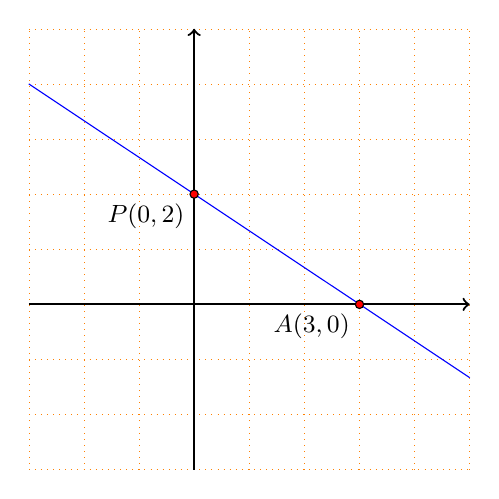
\begin{tikzpicture}[font=\small,x=7mm, y=7mm]

\draw[help lines,orange, dotted] (-3,-3) grid [step=1](5,5);

\begin{scope}[thick,->]
\draw (0,-3) -- (0,5);
\draw (-3,0) -- (5,0);
\end{scope}

\draw[blue] (-3,4) -- (5,-1.33);

\draw[fill=red] (0,2) circle (1.5pt) node[below left] {$P(0,2)$};
\draw[fill=red] (3,0) circle (1.5pt) node[below left] {$A(3,0)$};
\end{tikzpicture}% -----------------

% ---- fig043_ret.pgf ----
% (c) 2012 Dimitrios Vrettos - d.vrettos@gmail.com
\begin{tikzpicture}[font=\small,x=2mm, y=2mm]
	\draw (0,0) rectangle  (9.6,7.4);

\node [below left] at (0,0) {$A$};
\node[above left]  at (0,7.4) {$B$};
\node[below right]  at (9.6,0) {$D$};
\node[above right]  at (9.6,7.4) {$C$};
\end{tikzpicture}% -----------------

% ---- fig044_ese.pgf ----
% (c) 2012 Dimitrios Vrettos - d.vrettos@gmail.com
\begin{tikzpicture}[font=\small,x=10mm, y=10mm]
	\draw (0,0) --(8,0);

\node [below left] at (0,0) {$A$};
\node[below right]  at (8,0) {$B$};
\draw[fill=blue] (1.5,0) circle (1.5pt) node [below]  {$P$};

\end{tikzpicture}% -----------------

% ---- fig045_car.pgf ----
% (c) 2012 Dimitrios Vrettos - d.vrettos@gmail.com
% (c) 2012 Dimitrios Vrettos - d.vrettos@gmail.com
\begin{tikzpicture}[scale=.7, x=10mm, y=10mm]
    \draw[dotted,color=orange] (-3,-2) grid (8,7);
    \draw[->] (-3,0) -- (8,0) node[below left] {$x$};
    \draw[->] (0,-2) -- (0,7) node[below left] {$y$};
    
\foreach \x/\xtext in {-2/-2,-1/-1,1/1,2/2,3/3,4/4,5/5,6/6,7/7}
\node[below]  at (\x,0) {$\xtext$};
\foreach \y/\ytext in {-1/-1,1/1,2/2,3/3,4/4,5/5,6/6}
\node[left] at (0,\y) {$\ytext$};

\foreach \xi in {-2,-1,...,7}
\draw (\xi,3pt) -- (\xi,-3pt);
\foreach \yi in {-1,0,...,6}
\draw (3pt,\yi) -- (-3pt,\yi);

\node [below left] at (0,0) {0};
\draw[color=red,domain=-.5:7.2] plot[id=x] function{6-x} 
        node[right] {$a$};
    
\draw[color=blue,domain=1.3:3.4] plot[id=x] function{12-4*x} 
        node[right] {$b$};
  \draw[fill=green] (2,4) circle (1.5pt) node[above right] {$A(2,4)$};
\end{tikzpicture}% -----------------

% ---- fig046_car.pgf ----
% (c) 2012 Dimitrios Vrettos - d.vrettos@gmail.com
\begin{tikzpicture}[scale=.7, x=10mm, y=10mm]
    \draw[dotted,color=orange] (-4,-4) grid (5,4);
    \draw[->] (-4,0) -- (5,0) node[below left] {$x$};
    \draw[->] (0,-4) -- (0,4) node[below left] {$y$};
    
\foreach \x/\xtext in {-3/-3,-2/-2,-1/-1,1/1,2/2,3/3,4/4,}
\node[below]  at (\x,0) {$\xtext$};
\foreach \y/\ytext in {-3/-3,-2/-2,-1/-1,1/1,2/2,3/3}
\node[left] at (0,\y) {$\ytext$};

\foreach \xi in {-3,-2,...,4}
\draw (\xi,3pt) -- (\xi,-3pt);
\foreach \yi in {-3,-2,...,3}
\draw (3pt,\yi) -- (-3pt,\yi);

\node [below left] at (0,0) {0};
\draw[color=red,domain=-1.5:4.2] plot[id=x] function{(2*x-7)/3} 
        node[right] {$a$};
    
\draw[color=blue,domain=-3.5:4.2] plot[id=x] function{(2*x-3)/3} 
        node[right] {$b$};
\end{tikzpicture}% -----------------

% ---- fig047_car.pgf ----
% (c) 2012 Dimitrios Vrettos - d.vrettos@gmail.com
\begin{tikzpicture}[scale=.7, x=10mm, y=10mm]
    \draw[dotted,color=orange] (-4,-4) grid (5,3);
    \draw[->] (-4,0) -- (5,0) node[below left] {$x$};
    \draw[->] (0,-4) -- (0,3) node[below left] {$y$};
    
\foreach \x/\xtext in {-3/-3,-2/-2,-1/-1,1/1,2/2,3/3,4/4,}
\node[below]  at (\x,0) {$\xtext$};
\foreach \y/\ytext in {-3/-3,-2/-2,-1/-1,1/1,2/2}
\node[left] at (0,\y) {$\ytext$};

\foreach \xi in {-3,-2,...,4}
\draw (\xi,3pt) -- (\xi,-3pt);
\foreach \yi in {-3,-2,...,2}
\draw (3pt,\yi) -- (-3pt,\yi);

\node [below left] at (0,0) {0};
\draw[color=red,domain=-3.5:4.5] plot[id=x] function{-(2*x+1)/3} 
        node[right] {$a=b$};
\end{tikzpicture}% -----------------

% ---- lib_grafo3assi.pgf ----
% (c) 2014 Daniele Zambelli - daniele.zambelli@gmail.com

%%%
% Grafo per il calcolo del segno con tre assi
%%%%
 
\input{lbr/assiepiani/asse10x.pgf}
\begin{scope}[yshift= -.5cm]
  \input{lbr/assiepiani/asse10x.pgf}
  \begin{scope}[yshift= -.5cm]
    \input{lbr/assiepiani/asse10x.pgf}
  \end{scope}
\end{scope}

\draw [-] [] (a_top) -- (a_bottom);
\draw [-] [] (b_top) -- (b_bottom);
% -----------------

% ---- lib_grafo4assi.pgf ----
% (c) 2014 Daniele Zambelli - daniele.zambelli@gmail.com

%%%
% Grafo per il calcolo del segno con tre assi
%%%%
 
\input{lbr/assiepiani/asse10x.pgf}
\begin{scope}[yshift= -.5cm]
  \input{lbr/assiepiani/asse10x.pgf}
  \begin{scope}[yshift= -.5cm]
    \input{lbr/assiepiani/asse10x.pgf}
    \begin{scope}[yshift= -.5cm]
      \input{lbr/assiepiani/asse10x.pgf}
    \end{scope}
  \end{scope}
\end{scope}

\draw [-] [] (a_top) -- (a_bottom);
\draw [-] [] (b_top) -- (b_bottom);
\draw [-] [] (c_top) -- (c_bottom);
% -----------------

% ---- lib_rettacre.pgf ----
% (c) 2014 Daniele Zambelli - daniele.zambelli@gmail.com

%%%
% Retta crescente con segni
%%%%
 
\coordinate (inizio) at (-10, -4);
\coordinate (zero) at (0, 0);
\coordinate (fine) at (10, 4);

\input{lbr/assiepiani/asse10x.pgf}

\draw [-] [ultra thick, red!50!black] (inizio) -- (zero);
\draw [-] [ultra thick, blue!50!black] (zero) -- (fine);

\node [xshift=-25, yshift=-3, above] at (zero) {$-$};
\draw[blue, thick, fill=white] (zero) circle (2pt);
\node [xshift=25, yshift=-3, above] at (zero) {$+$};
% -----------------

% ---- lib_rettadec.pgf ----
% (c) 2014 Daniele Zambelli - daniele.zambelli@gmail.com

%%%
% Retta decrescente con segni
%%%%
 
\coordinate (inizio) at (-10, 4);
\coordinate (zero) at (0, 0);
\coordinate (fine) at (10, -4);

\input{lbr/assiepiani/asse10x.pgf}

\draw [-] [ultra thick, blue!50!black] (inizio) -- (zero);
\draw [-] [ultra thick, red!50!black] (zero) -- (fine);

\node [xshift=-25, yshift=-3, above] at (zero) {$+$};
\draw[blue, thick, fill=white] (zero) circle (2pt);
\node [xshift=25, yshift=-3, above] at (zero) {$-$};
% -----------------
